% AutoRL manuscript (LaTeX)
% Generated for the AutoRL workspace

\documentclass[11pt]{article}

\usepackage[margin=1in]{geometry}
\usepackage{amsmath, amssymb, amsfonts}
\usepackage{booktabs}
\usepackage{siunitx}
\usepackage{graphicx}
\usepackage{hyperref}
\usepackage[nameinlink,noabbrev]{cleveref}

\hypersetup{
  colorlinks=true,
  linkcolor=blue,
  citecolor=blue,
  urlcolor=blue
}

\title{AutoRL for Predictive Maintenance on the Edge: \texorpdfstring{\newline}{ }A Comparative Study of REINFORCE with Attention Mechanisms for Milling Tool Replacement}

\author{Rajesh Siraskar\\
\small PhD Researcher, Predictive Maintenance and Reinforcement Learning\\
\small (Affiliation as appropriate)\\
\small \texttt{(email as appropriate)}
}

\date{March 2026}

\begin{document}
\maketitle

\begin{abstract}
Industry~4.0 maintenance systems increasingly rely on edge-computing deployments where stringent limits on memory, latency, and energy consumption favor computationally light learning methods. In this work we study \emph{AutoRL}, an automated reinforcement learning (RL) pipeline that trains and evaluates maintenance agents for a milling machine tool-replacement task, with particular focus on whether the na\"{i}ve Monte-Carlo policy-gradient algorithm \textsc{REINFORCE} can be competitive with more advanced methods such as \textsc{PPO}. The contribution is threefold: (i) an end-to-end AutoRL training and multi-round evaluation framework, (ii) a Gymnasium-compatible predictive-maintenance environment that hides tool wear from observations to enforce inference from sensor signals alone, and (iii) a systematic comparison across four RL algorithms (\textsc{A2C}, \textsc{DQN}, \textsc{PPO}, \textsc{REINFORCE}) and four attention mechanisms (Nadaraya--Watson, Temporal, Multi-Head, Self-Attention) integrated as Stable-Baselines3 feature extractors.

Across 48 trained agents (3 training files $\times$ 4 algorithms $\times$ 4 attention mechanisms) and 20 evaluation rounds per configuration, tested on six unseen datasets, \textsc{REINFORCE} with temporal or multi-head attention achieves the highest mean evaluation score and is statistically superior to non-\textsc{REINFORCE} baselines (one-tailed Welch $t$-test, $p\ll 0.05$). The results suggest that, when paired with inductive biases from attention feature extractors, lightweight policy-gradient methods can match (and sometimes exceed) heavier optimization schemes while aligning with sustainability and carbon-footprint objectives.
\end{abstract}

\textbf{Keywords:} Predictive maintenance; Industry~4.0; Edge computing; Reinforcement learning; \textsc{REINFORCE}; \textsc{PPO}; Attention mechanisms; Milling machine; Sustainable AI.

\section{Context: Industry~4.0/5.0, predictive maintenance, and edge constraints}
Predictive maintenance (PdM) is a foundational Industry~4.0 capability: instrumented assets continuously produce sensor telemetry and maintenance decisions are optimized to reduce unplanned downtime and extend component life. In practical deployments, PdM must increasingly operate at the \emph{edge}---near machines and shop-floor controllers---to meet latency, bandwidth, and reliability constraints, and to reduce operational risk associated with centralized compute.

Edge deployment imposes hard resource limits (compute cycles, memory footprint, and energy), motivating \emph{lightweight} ML/RL models and training procedures. These constraints directly relate to sustainability considerations: lower compute and shorter training runs reduce electricity consumption and associated carbon emissions, which is increasingly relevant in corporate carbon accounting and Industry~5.0 human-centric and sustainable manufacturing initiatives. Recent work in ``Green AI'' emphasizes reporting and minimizing computational cost as a first-class metric alongside accuracy~\cite{Schwartz2020GreenAI, Strubell2019Energy}.

Beyond operational cost, reducing computational demand supports organizational carbon-footprint targets and can strengthen evidence bases used in carbon-credit and ESG reporting workflows, making ``efficient learning'' practically consequential rather than purely academic.

In this setting, a key research question emerges:
\begin{quote}
\emph{Can simple, computationally light RL algorithms such as \textsc{REINFORCE} be competitive with more advanced policy-optimization methods (e.g., \textsc{PPO}) for PdM decision-making, especially when augmented with attention-based feature extraction?}
\end{quote}

This study builds directly on prior findings that na\"{i}ve \textsc{REINFORCE} can perform strongly for PdM in untuned regimes and that automated RL frameworks can help industrial practitioners explore algorithm--hyperparameter design spaces~\cite{Siraskar2025NaiveREINFORCE}. It also leverages prior work applying a Nadaraya--Watson estimator as a lightweight attention mechanism for PdM, motivated by edge constraints~\cite{Siraskar2024NWAttention}.

\section{AutoRL overview}
\subsection{Motivation and design goals}
AutoRL is designed as a practical experimentation platform to (i) train multiple RL agents over a grid of algorithmic choices and hyperparameters, (ii) evaluate agents on multiple test files using prognostic-aware metrics, and (iii) generate standard plots (heatmaps and analysis summaries) for model selection.

The implementation in this repository provides both a Streamlit application and a CLI pipeline. The CLI (\texttt{train\_agent.py}) supports training, discovery of trained models, and evaluation in single-round or multi-round modes. Multi-round evaluation produces a ``long'' CSV with all repetitions to enable statistical analysis (e.g., $t$-tests).

\subsection{Experimental automation and reproducibility}
The pipeline supports:
\begin{itemize}
  \item training across algorithms and attention types (feature extractor plug-ins),
  \item evaluation across multiple datasets with repeated rounds (here: 20 rounds),
  \item checkpointing and retry logic using a lightweight SQLite queue to recover from failures during long experiments.
\end{itemize}

In addition to model files, each trained agent writes a metadata JSON containing algorithm, attention mechanism, training file, learning rate, discount factor, number of episodes, and training summaries.

\section{Predictive maintenance as a Markov decision process}
\subsection{MDP and POMDP formulation}
We model the maintenance decision problem as an episodic Markov decision process (MDP) $\mathcal{M}=(\mathcal{S},\mathcal{A},P,r,\gamma)$~\cite{SuttonBarto2018}, where $\mathcal{S}$ is the set of environment states, $\mathcal{A}$ is the action space, $P$ is the transition kernel, $r$ is the reward function, and $\gamma$ is the discount factor. At each discrete timestep $t$, the agent chooses an action
\begin{equation}
  a_t \in \mathcal{A}=\{0,1\},
\end{equation}
where $a_t=0$ denotes \emph{replace} and $a_t=1$ denotes \emph{continue}. The environment evolves along a recorded run-to-failure dataset where the latent degradation variable (tool wear) is $w_t$.

\paragraph{Hidden states and partial observability.}
In classical MDPs, the agent observes the full state $s_t$ at each step. However, in real-world predictive maintenance, the true state (e.g., tool wear $w_t$) is often \emph{hidden} and cannot be measured directly. Instead, the agent receives a partial observation $o_t$ derived from sensor signals. This setting is more accurately described as a \emph{partially observable MDP} (POMDP), defined by $\mathcal{M}'=(\mathcal{S},\mathcal{A},P,r,\gamma,\mathcal{O},O)$, where $\mathcal{O}$ is the observation space and $O$ is the observation function:
\begin{equation}
  o_t = O(s_t) = \mathrm{Sensors}(t), \qquad w_t \notin o_t.
\end{equation}
The agent must infer the hidden state (wear) from the history of observations and actions, motivating the use of feature extractors and attention mechanisms to capture temporal and cross-sensor dependencies.

\subsection{Observation design: wear is hidden}
A critical modelling choice is that $w_t$ is \emph{excluded} from observations. The agent must infer maintenance decisions solely from sensors (forces, vibrations, acoustics, currents), which aligns with realistic deployments where true wear is expensive or impossible to measure in real time. Formally, the observation is as above:
\begin{equation}
  o_t \equiv \mathbf{x}_t = \mathrm{Sensors}(t),\qquad w_t\notin o_t.
\end{equation}
This makes the environment a simple POMDP, not a fully observable MDP. The state is only partially visible, and the agent must learn to extract relevant information from the available sensor data.

\subsection{Episode termination}
Episodes terminate on (i) action \emph{replace} or (ii) a threshold violation (wear exceeding the wear threshold), or (iii) end-of-file truncation.

\subsection{Reward function}
The reward is shaped to encourage (a) long tool usage without violation and (b) replacement close to (but before) the wear threshold. With wear threshold $W$ and wear ratio $\rho_t=w_t/W$, the environment implements a piecewise reward (see \texttt{MT\_Env.step} in \texttt{rl\_pdm.py}):
\begin{align}
  r_t =
  \begin{cases}
    R_3 + \kappa(\rho_t) & a_t=0,\; w_t\le W \\
    \tfrac{1}{2}R_2 & a_t=0,\; w_t>W \\
    R_2 & a_t=1,\; w_t>W \\
    R_1 & a_t=1,\; w_t\le W
  \end{cases}
\end{align}
where $R_1$ is a small survival reward, $R_2$ is a catastrophic violation penalty, $R_3$ is a small replacement cost, and $\kappa(\rho)$ is a bonus increasing with $\rho$ for high-wear pre-threshold replacement (implemented as a stepped function for $\rho>0.7,0.8,0.9$).

This design encodes an asymmetric risk profile consistent with safety-critical maintenance: a single violation is substantially worse than an ``early'' replacement.

\section{Attention mechanisms for predictive maintenance}
\subsection{Attention in general}
Attention mechanisms allow models to dynamically focus on the most relevant parts of their input. In its general form, attention is a mapping from queries $Q$, keys $K$, and values $V$ to a context representation:
\begin{equation}
  \mathrm{Att}(Q,K,V) = \mathrm{softmax}\!\left(\frac{QK^\top}{\sqrt{d_k}}\right)V,
\end{equation}
where $d_k$ is the key dimension. This formulation, popularized by Transformer architectures~\cite{Vaswani2017Attention}, enables the model to weigh different input features or time steps according to their relevance.

In predictive maintenance, attention is attractive because it can (i) emphasize salient sensors, (ii) highlight interactions among signals, and (iii) provide a structured inductive bias without necessarily increasing end-to-end model complexity dramatically. In this work, attention is implemented as a \emph{feature extractor} $\phi_\theta(\mathbf{x}_t)$ inside the policy/value networks (Stable-Baselines3 custom extractors), shifting attention from ``sequence-to-sequence'' NLP settings to ``feature weighting/fusion'' over multi-sensor inputs.

\subsection{Nadaraya--Watson (NW) attention}
\paragraph{Theory.}
The Nadaraya--Watson estimator performs kernel regression by computing a similarity-weighted average over reference points~\cite{Nadaraya1964, Watson1964}. In an attention view, the query is the current feature vector and keys are prototypes; weights are derived from a kernel over distances.

\paragraph{Implementation in AutoRL.}
The extractor (\texttt{NadarayaWatsonExtractor}) learns:
(i) a positive bandwidth parameter $\beta=\exp(\log\beta)$,
(ii) a set of learnable keys $\{\mathbf{k}_i\}_{i=1}^m$ and values $\{\mathbf{v}_i\}_{i=1}^m$ (memory/prototypes), and
(iii) a linear query projection.
For a batch element, the attention weights are
\begin{equation}
  \alpha_i = \mathrm{softmax}\bigl(-\beta\,\lVert \mathbf{q}-\mathbf{k}_i\rVert_2^2\bigr),
\end{equation}
and the output context is $\sum_i \alpha_i\mathbf{v}_i$.

\paragraph{Pros/cons.}
NW attention is computationally light (distance + softmax), offers a smooth inductive bias, and connects to prior PdM attention work emphasizing edge constraints~\cite{Siraskar2024NWAttention}. However, prototype-based memories may underfit complex feature interactions when the optimal policy depends on higher-order relationships across sensors.

\subsection{Temporal attention (TP)}
\paragraph{Theory.}
Degradation is inherently temporal; positional encodings provide a simple mechanism to inject time context into a feed-forward representation. Sinusoidal encodings are defined as
\begin{align}
  \mathrm{PE}(pos,2i) &= \sin\left(\frac{pos}{10000^{2i/d}}\right),\\
  \mathrm{PE}(pos,2i{+}1) &= \cos\left(\frac{pos}{10000^{2i/d}}\right).
\end{align}

\paragraph{Implementation in AutoRL.}
The extractor (\texttt{TemporalAttentionExtractor}) uses: (i) a fixed sinusoidal positional encoding buffer, (ii) a learnable temporal embedding vector, (iii) a spatial attention MLP producing a per-feature soft mask, and (iv) a fusion MLP over concatenated weighted spatial features and temporal features. A timestep counter is maintained as a buffer and incremented on each forward pass.

\paragraph{Pros/cons.}
Temporal attention is lightweight yet adds an explicit monotone-time context, which is often missing in per-timestep sensor vectors. A limitation is that the internal timestep is not automatically reset by the policy network on environment resets; care must be taken in production to align temporal state with episode boundaries.

\subsection{Multi-head attention (MH)}
\paragraph{Theory.}
Multi-head attention typically learns multiple subspaces of attention to capture heterogeneous dependencies~\cite{Vaswani2017Attention}.

\paragraph{Implementation in AutoRL.}
The extractor (\texttt{MultiHeadAttentionExtractor}) projects the observation into queries, keys, and values and reshapes them into $H$ heads. Because observations are single feature vectors (not sequences), the code computes a per-head scalar score
\begin{equation}
  s_h = \frac{\langle \mathbf{Q}_h, \mathbf{K}_h\rangle}{\sqrt{d_h}},\qquad
  \alpha_h = \mathrm{softmax}(\mathbf{s})_h,
\end{equation}
then gates each head's value $\mathbf{V}_h$ by $\alpha_h$ and concatenates across heads. This acts as a structured mixture-of-subspaces: different heads can specialize to different sensor groupings or degradation regimes.

\paragraph{Pros/cons.}
MH adds representational capacity with controlled width and can be efficient on low-dimensional sensor vectors. Since attention is over heads rather than over time indices, interpretability differs from classical temporal self-attention.

\subsection{Self-attention (SA)}
\paragraph{Theory.}
Self-attention is a mechanism that allows each feature (or token) to attend to all others, learning dependencies and interactions. In the standard Transformer, self-attention is defined as:
\begin{equation}
  \mathrm{SelfAtt}(X) = \mathrm{softmax}\left(\frac{XW_Q (XW_K)^\top}{\sqrt{d_k}}\right) XW_V
\end{equation}
where $X \in \mathbb{R}^{n \times d}$ is the input (with $n$ features or tokens), and $W_Q, W_K, W_V$ are learned projection matrices. This computes a weighted sum of value vectors for each feature, with weights determined by the similarity of queries and keys.

In our setting, the input $X$ is a batch of projected sensor feature vectors (not a sequence), so self-attention operates across features or across the batch, depending on implementation. This enables the model to learn complex relationships between sensor channels.

\paragraph{Implementation in AutoRL.}
The extractor (\texttt{SelfAttentionExtractor}) projects inputs to a feature space and computes $Q,K,V$ with linear layers. It forms a scalar score via a dot product and applies a softmax normalization across the \emph{batch} dimension, then uses residual connections and a feed-forward network with layer normalization. The batchwise normalization acts as a gating mechanism, but is not equivalent to standard token-wise attention.

\paragraph{Pros/cons.}
This design can stabilize training via normalization and residual structure, and can model feature interactions. However, batchwise normalization may introduce sensitivity to batch composition and is less interpretable than classical temporal self-attention.

\section{RL algorithms studied}
We compare four standard RL approaches commonly used for control and decision-making.

\subsection{\textsc{DQN}}
\textsc{DQN} learns an action-value function $Q_\theta(s,a)$ and minimizes a temporal-difference objective~\cite{Mnih2015DQN}:
\begin{equation}
  \mathcal{L}(\theta) = \mathbb{E}\bigl[\bigl(r_t + \gamma \max_{a'}Q_{\bar\theta}(s_{t+1},a') - Q_\theta(s_t,a_t)\bigr)^2\bigr],
\end{equation}
where $\bar\theta$ denotes a target network.

\subsection{\textsc{A2C}}
Actor--critic methods learn both a policy $\pi_\theta(a|s)$ and a value baseline $V_\psi(s)$. The advantage estimate
\begin{equation}
  \hat{A}_t = \hat{G}_t - V_\psi(s_t)
\end{equation}
reduces variance in policy gradients. \textsc{A2C} is a synchronous variant of the asynchronous actor--critic family~\cite{Mnih2016A3C}.

\subsection{\textsc{PPO}}
\textsc{PPO} improves stability by constraining policy updates via a clipped surrogate objective~\cite{Schulman2017PPO}:
\begin{align}
  r_t(\theta) &= \frac{\pi_\theta(a_t|s_t)}{\pi_{\theta_{\text{old}}}(a_t|s_t)},\\
  \mathcal{L}^{\text{clip}}(\theta) &= \mathbb{E}\left[\min\Big(r_t(\theta)\hat{A}_t,\; \mathrm{clip}(r_t(\theta),1{-}\epsilon,1{+}\epsilon)\hat{A}_t\Big)\right].
\end{align}
While effective, PPO typically incurs higher compute due to multiple epochs/minibatch passes per batch.

\subsection{\textsc{REINFORCE}}
\textsc{REINFORCE}~\cite{Williams1992REINFORCE} estimates the policy gradient from Monte-Carlo returns. For a trajectory $\tau=(s_0,a_0,\dots,s_T)$ with return
\begin{equation}
  G_t = \sum_{k=0}^{T-t-1}\gamma^k r_{t+k},
\end{equation}
REINFORCE performs gradient ascent on
\begin{equation}
  J(\theta) = \mathbb{E}_{\tau\sim \pi_\theta}\left[\sum_{t=0}^{T-1} G_t\right],
\end{equation}
with gradient estimator
\begin{equation}
  \nabla_\theta J(\theta) \approx \mathbb{E}\left[\sum_{t=0}^{T-1} \nabla_\theta \log \pi_\theta(a_t|s_t)\, (G_t - b(s_t))\right].
\end{equation}

\paragraph{Implementation in AutoRL.}
The code implements an SB3-compatible \texttt{REINFORCE} class that uses the SB3 rollout buffer returns and an optional value-function baseline (\texttt{use\_baseline=True}). The loss corresponds to
\begin{equation}
  \mathcal{L}(\theta,\psi)= -\mathbb{E}[\log\pi_\theta(a|s)\,\hat{A}] + \lambda_H\,\mathcal{L}_{\text{ent}} + \lambda_V\,\lVert \hat{G} - V_\psi(s)\rVert_2^2,
\end{equation}
where entropy regularization encourages exploration.

\paragraph{Why \textsc{REINFORCE} can be edge-suited.}
Compared to PPO, REINFORCE is algorithmically simpler (no ratio clipping, fewer inner optimization epochs) and thus can reduce training-side compute. In an AutoRL setting where many algorithm/attention combinations are trained, such savings compound and can lower overall experimental carbon footprint.

\section{Evaluation metrics}
\subsection{Prognostic-specific $\lambda$ metric}
PdM evaluation requires metrics beyond generic RL return. Following the prognostics-oriented evaluation perspective synthesized in a systematic technical review~\cite{RLforPdMReview2023}, we use a $\lambda$-style timing metric derived from the time difference between a model's first replacement prediction and a threshold-based ``end-of-life'' point.

In code, the environment defines an ``in-advance replacement'' (IAR) window around the wear threshold $W$ with range parameter $\eta$ (\texttt{IAR\_RANGE}=0.05). The IAR lower bound is
\begin{equation}
  w_{\text{IAR}} = W(1-\eta),
\end{equation}
and $t_\lambda$ is the first timestep where $w_t\ge w_{\text{IAR}}$. Let $t_{\text{FR}}$ be the first timestep where the agent chooses \emph{replace}. The signed timing metric is
\begin{equation}
  \lambda = t_\lambda - t_{\text{FR}},
\end{equation}
and the evaluation normalizes $|\lambda|$ so that smaller values are better.

\subsection{Composite evaluation score}
To compare policies, AutoRL defines a normalized weighted score (\texttt{calculate\_eval\_score}):
\begin{equation}
  S = 0.50\,S_U + 0.30\,S_\lambda + 0.20\,S_V, \qquad S\in[0,1],
\end{equation}
where $S_U$ is normalized tool usage, $S_\lambda = \max\{0,1-|\lambda|/w_{\text{IAR}}\}$, and $S_V=1/(1+\text{violations})$ penalizes threshold violations.

\section{Experimental setup}
\subsection{Datasets and generalization protocol}
Experiments use the SIT milling-machine sensor schema (8 sensor channels per timestep). Models are trained on three files (\texttt{SIT\_8}, \texttt{SIT\_10}, \texttt{SIT\_12}) and evaluated on six unseen files (\texttt{SIT\_7}, \texttt{SIT\_9}, \texttt{SIT\_11}, \texttt{SIT\_13}, \texttt{SIT\_14}, \texttt{SIT\_15}). This split supports a domain-generalization question: does a learned maintenance policy transfer to unseen runs?

\subsection{Model grid}
We train $3\times 4\times 4 = 48$ agents: algorithms \{\textsc{A2C}, \textsc{DQN}, \textsc{PPO}, \textsc{REINFORCE}\} crossed with attention types \{NW, TP, MH, SA\}. Training metadata indicates $500$ episodes, learning rate $10^{-4}$, and $\gamma=0.99$ for the reported model set.

\subsection{Multi-round evaluation}
Each model--test-file pair is evaluated for 20 rounds. The long-form results CSV is retained for statistical analysis; plots and heatmaps use round means. The primary analysis artifacts used in this paper are:
\begin{itemize}
  \item \texttt{results/Analysis/01-Mar-2026 Good Set-1/Evaluation\_Results\_Multiround\_SIT\_NoAM\_20260301\_181435.csv},
  \item \texttt{paper/figures/analysis\_report\_sit.png},
  \item \texttt{paper/figures/heatmap\_allagents\_sit.png}.
\end{itemize}

\section{Results}
\subsection{Overall performance and best configurations}
\Cref{fig:analysisreport} and \Cref{fig:heatmap} summarize the evaluation outcomes. The top-performing combinations on unseen test files are \textsc{REINFORCE}+Temporal and \textsc{REINFORCE}+Multi-Head, both achieving mean evaluation score $\approx 0.947$ with tight confidence intervals.

\begin{table}[t]
\centering
\caption{Top configurations on \emph{unseen} test files (mean $\pm$ 95\% CI, 20 rounds; $n=360$ rows per configuration).}
\label{tab:top}
\sisetup{round-mode=places,round-precision=3}
\begin{tabular}{ll S[table-format=1.3] S[table-format=1.3] S[table-format=2.3] S[table-format=3.3]}
\toprule
\textbf{Algorithm} & \textbf{Attention} & {\textbf{Eval. Score}} & {\textbf{CI}} & {\textbf{Tool use (\%)}} & {\textbf{$\lambda$}} \\
\midrule
REINFORCE & Temporal   & 0.947 & 0.002 & 95.661 & -30.000 \\
REINFORCE & Multi-Head & 0.946 & 0.002 & 95.661 & -30.333 \\
PPO       & Multi-Head & 0.946 & 0.002 & 95.661 & -30.444 \\
PPO       & Temporal   & 0.732 & 0.032 & 81.171 & 113.444 \\
PPO       & NW         & 0.729 & 0.032 & 81.482 & 109.389 \\
\bottomrule
\end{tabular}
\end{table}

\subsection{Hypothesis testing: is REINFORCE better?}
To quantify whether \textsc{REINFORCE} improves the evaluation score distribution, we perform a one-tailed independent Welch $t$-test comparing \textsc{REINFORCE} scores against all non-\textsc{REINFORCE} scores (implemented in \texttt{Hypotheis\_test.ipynb}). The test yields $t=22.70$ and $p=1.70\times 10^{-90}$ at $\alpha=0.05$, rejecting $H_0$ in favor of $H_1$: \textsc{REINFORCE} is significantly better on this evaluation distribution.

\subsection{Why REINFORCE + (MH/TP) can match or exceed PPO}
Empirically, the top three configurations are within a narrow band (Table~\ref{tab:top}). We propose the following mechanisms explaining why \textsc{REINFORCE}+MH/TP can be comparable to \textsc{PPO} in this setting:
\begin{itemize}
  \item \textbf{Inductive bias dominates optimizer sophistication.} When wear is hidden, the primary challenge is representation learning from sensors. MH and TP extractors inject structure (subspace gating and time-context fusion), reducing the burden on the policy optimizer.
  \item \textbf{Small action space and short-horizon decision.} With $|\mathcal{A}|=2$ and termination on replacement, the control problem can be closer to learning a boundary in feature space than to long-horizon continuous control, reducing the relative advantage of PPO-style constrained updates.
  \item \textbf{Variance reduction via baseline.} Although termed ``na\"{i}ve'', the implementation uses a value-function baseline (by default) which reduces gradient variance and can yield stable learning.
  \item \textbf{Compute-efficiency and AutoRL scaling.} Because PPO typically performs multiple epochs per batch, AutoRL-style sweeps amplify PPO compute. REINFORCE offers a favorable trade-off when many configurations must be explored.
\end{itemize}

\section{Discussion: implications for edge computing and sustainability}
The strongest-performing configurations combine high tool-use (\(\approx 95.7\%\)) with near-zero violations and low normalized $|\lambda|$. Importantly, these results are achieved with an algorithmically simple policy-gradient method, reinforcing the argument that lightweight RL is a viable candidate for edge-focused PdM.

From a sustainability perspective, algorithmic simplicity matters: when AutoRL frameworks are used as practitioner-facing platforms, reducing the compute per experiment reduces the overall energy footprint of the exploration process~\cite{Schwartz2020GreenAI}. This aligns with Industry~4.0/5.0 trajectories where operational excellence and environmental responsibility are jointly optimized.

\section{Limitations and future work}
This study is intentionally scoped to a dataset-driven episodic environment. Future work should:
\begin{itemize}
  \item evaluate deployment-centric metrics (model size, inference latency, energy) on representative edge hardware,
  \item refine temporal-state handling in temporal extractors (explicit reset on episode boundaries),
  \item validate robustness under sensor noise, drift, and domain shift across machines.
\end{itemize}

\section{Conclusion}
We presented AutoRL, a reproducible pipeline for training and evaluating PdM RL agents with attention-based feature extraction. The experimental evidence on SIT milling data demonstrates that \textsc{REINFORCE} paired with temporal or multi-head attention is competitive with (and in aggregate outperforms) \textsc{PPO} and other baselines, while preserving algorithmic simplicity desirable for edge-computing and sustainable AI goals.

\section*{Code and data availability}
This manuscript is based on the accompanying AutoRL codebase (\texttt{train\_agent.py}, \texttt{rl\_pdm.py}) and the evaluation artifacts under \texttt{results/Analysis/}.

\begin{figure}[t]
\centering
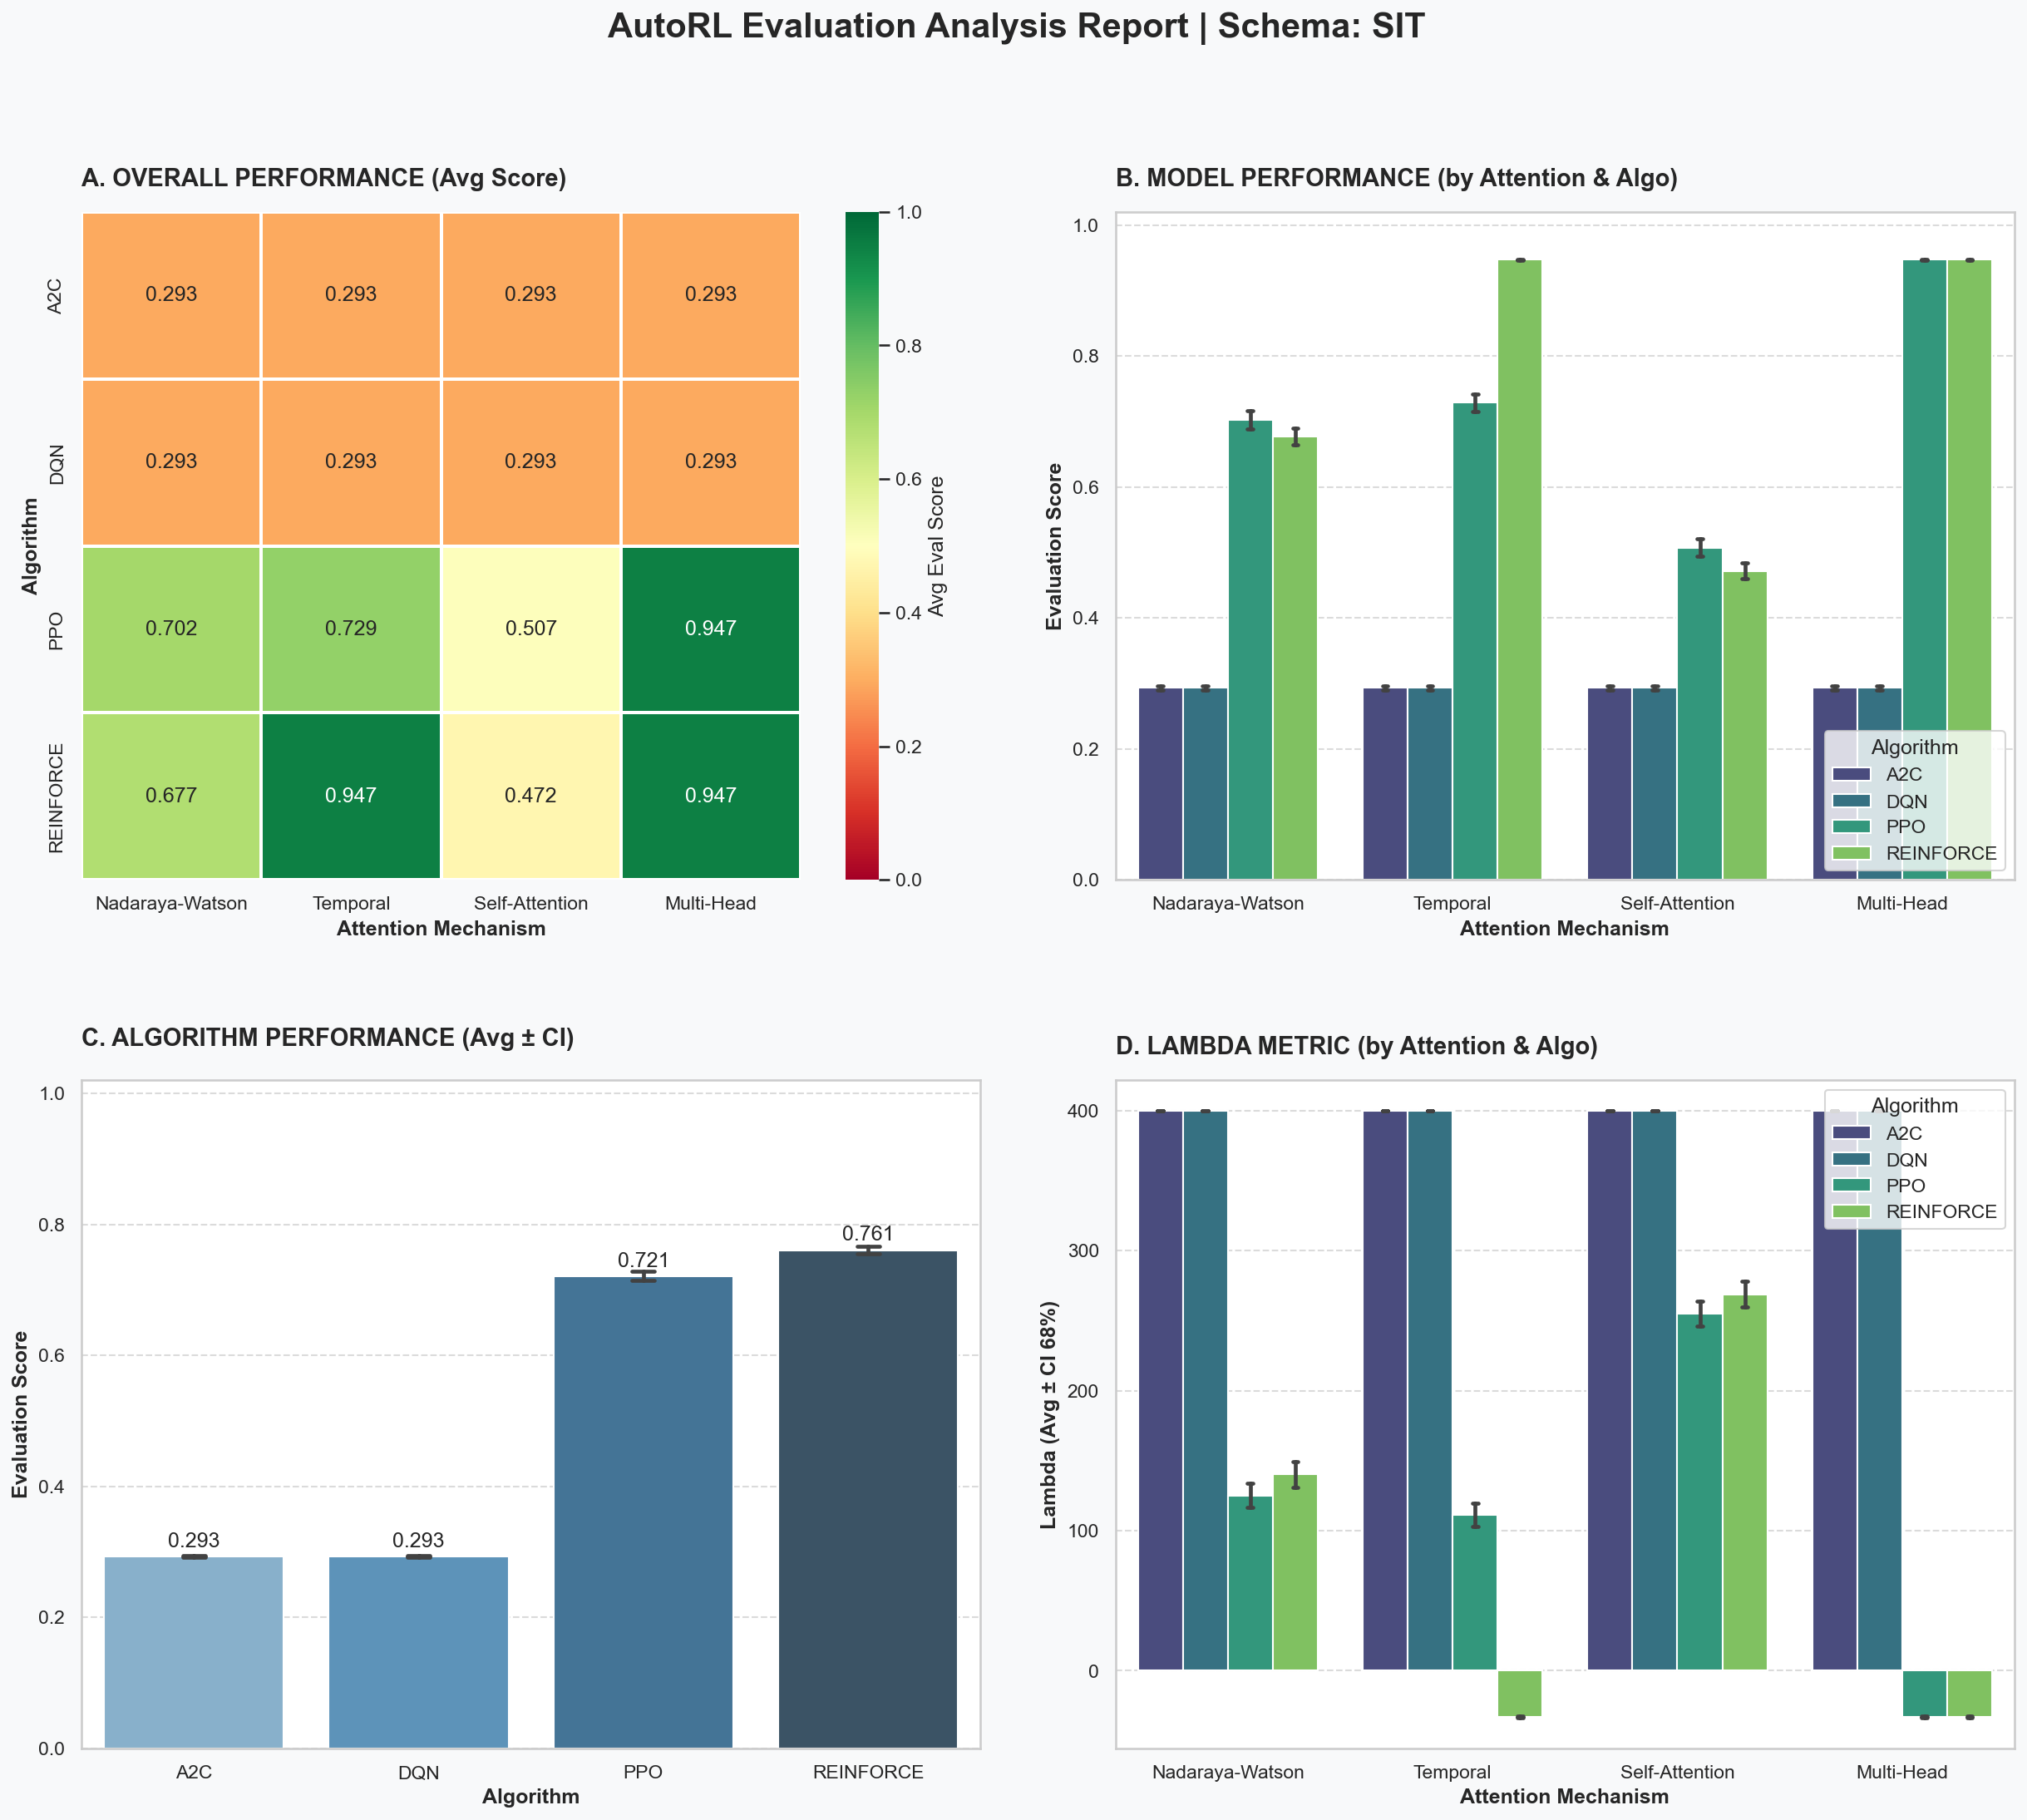
\includegraphics[width=\linewidth]{paper/figures/analysis_report_sit.png}
\caption{AutoRL evaluation analysis report (SIT schema). Panels summarize (A) mean evaluation score across algorithms and attention mechanisms, (B) grouped comparisons, (C) algorithm-level means with confidence intervals, and (D) the $\lambda$ metric.}
\label{fig:analysisreport}
\end{figure}

\begin{figure}[t]
\centering
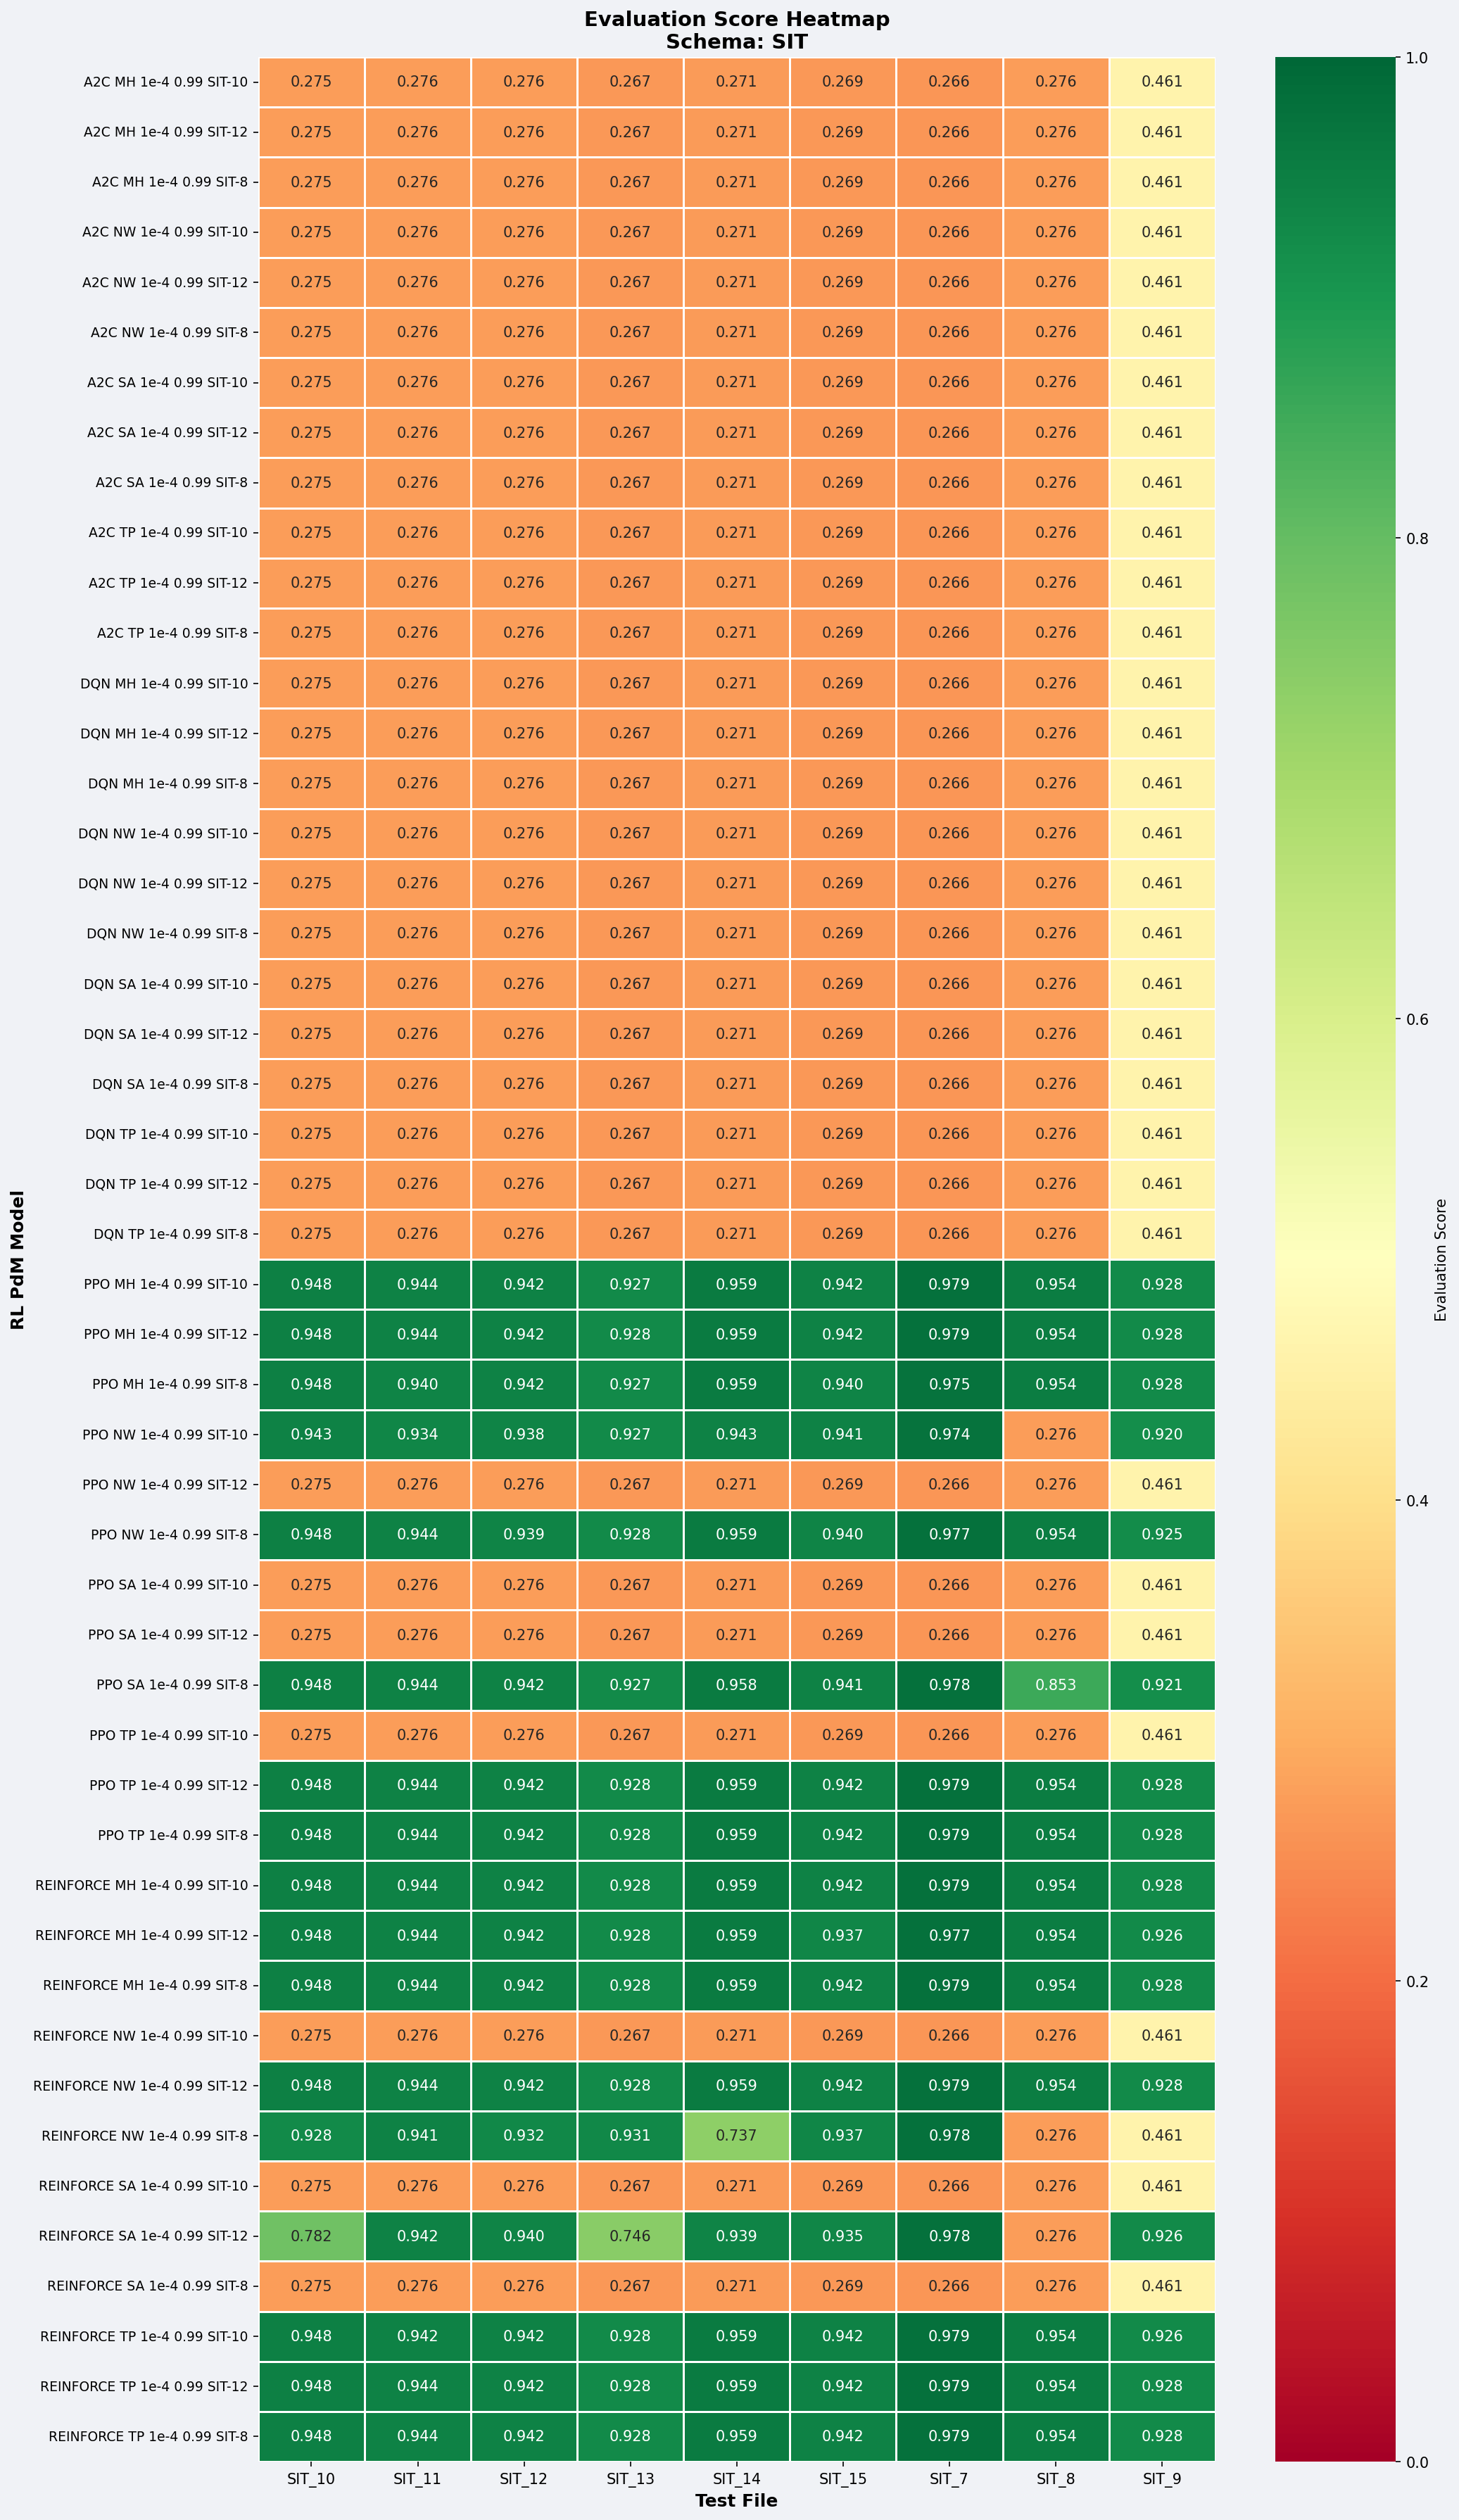
\includegraphics[width=\linewidth]{paper/figures/heatmap_allagents_sit.png}
\caption{Heatmap of evaluation scores across trained agent configurations (SIT schema). Each row corresponds to an RL model variant; columns are test files. The best-performing region corresponds to \textsc{REINFORCE} with multi-head or temporal attention.}
\label{fig:heatmap}
\end{figure}

\begin{thebibliography}{99}

\bibitem{SuttonBarto2018}
R.~S. Sutton and A.~G. Barto.
\newblock \emph{Reinforcement Learning: An Introduction}.
\newblock MIT Press, 2nd edition, 2018.

\bibitem{Williams1992REINFORCE}
R.~J. Williams.
\newblock Simple statistical gradient-following algorithms for connectionist reinforcement learning.
\newblock \emph{Machine Learning}, 8:229--256, 1992.

\bibitem{Mnih2015DQN}
V.~Mnih et~al.
\newblock Human-level control through deep reinforcement learning.
\newblock \emph{Nature}, 518:529--533, 2015.

\bibitem{Mnih2016A3C}
V.~Mnih et~al.
\newblock Asynchronous methods for deep reinforcement learning.
\newblock \emph{Proceedings of ICML}, 2016.

\bibitem{Schulman2017PPO}
J.~Schulman, F.~Wolski, P.~Dhariwal, A.~Radford, and O.~Klimov.
\newblock Proximal policy optimization algorithms.
\newblock \emph{arXiv:1707.06347}, 2017.

\bibitem{Vaswani2017Attention}
A.~Vaswani et~al.
\newblock Attention is all you need.
\newblock \emph{Advances in Neural Information Processing Systems (NeurIPS)}, 2017.

\bibitem{Nadaraya1964}
E.~A. Nadaraya.
\newblock On estimating regression.
\newblock \emph{Theory of Probability and Its Applications}, 9(1):141--142, 1964.

\bibitem{Watson1964}
G.~S. Watson.
\newblock Smooth regression analysis.
\newblock \emph{Sankhy\={a}: The Indian Journal of Statistics, Series A}, pages 359--372, 1964.

\bibitem{Schwartz2020GreenAI}
R.~Schwartz, J.~Dodge, N.~A. Smith, and O.~Etzioni.
\newblock Green {AI}.
\newblock \emph{Communications of the ACM}, 63(12):54--63, 2020.

\bibitem{Strubell2019Energy}
E.~Strubell, A.~Ganesh, and A.~McCallum.
\newblock Energy and policy considerations for deep learning in {NLP}.
\newblock \emph{Proceedings of ACL}, 2019.

\bibitem{Siraskar2025NaiveREINFORCE}
R.~Siraskar.
\newblock An empirical study of the na\"{i}ve {REINFORCE} algorithm for predictive maintenance.
\newblock \emph{Discover Applied Sciences}, 2025.
\newblock DOI: \href{https://doi.org/10.1007/s42452-025-06613-1}{10.1007/s42452-025-06613-1}.

\bibitem{Siraskar2024NWAttention}
R.~Siraskar, S.~Kumar, S.~Patil, A.~Bongale, and K.~Kotecha.
\newblock Application of the {Nadaraya--Watson} estimator based attention mechanism to the field of predictive maintenance.
\newblock \emph{MethodsX}, 12:102754, 2024.
\newblock DOI: \href{https://doi.org/10.1016/j.mex.2024.102754}{10.1016/j.mex.2024.102754}.

\bibitem{RLforPdMReview2023}
Reinforcement learning for predictive maintenance: a systematic technical review.
\newblock \emph{Artificial Intelligence Review}, 2023.
\newblock DOI: \href{https://doi.org/10.1007/s10462-023-10468-6}{10.1007/s10462-023-10468-6}.

\bibitem{Raffin2021SB3}
A.~Raffin et~al.
\newblock Stable-baselines3: Reliable reinforcement learning implementations.
\newblock \emph{Journal of Machine Learning Research}, 22(268):1--8, 2021.

\end{thebibliography}

\end{document}
